出力予測モデルである$y$は入力$x$とパラメータ$\Theta$によって変わる. したがって, $Theta$が異なると様々な予測モデルができる.
\begin{center}
    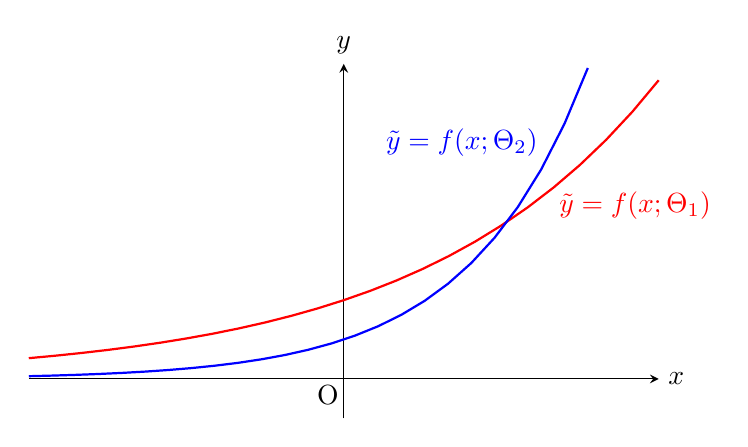
\begin{tikzpicture}[>=stealth]
        \draw[->](-4,0)--(4,0) node[right] {$x$};
        \draw[->](0,-0.5)--(0,4) node[above]{$y$};
        \node at(-0.2,-0.2) {O};
        \draw[draw=red,thick,domain=-4:4] plot(\x,{exp(\x/3)});
        \draw[draw=blue,thick,domain=-4:3.1] plot(\x,{exp(\x/1.5)/2});
        \node at(3.7,2.2) {\textcolor{red}{$\tilde{y}=f(x;\Theta_{1})$}};
        \node at(1.5,3) {\textcolor{blue}{$\tilde{y}=f(x;\Theta_{2})$}};
    \end{tikzpicture}
\end{center}
このようなモデルに対して学習データ(training data)を用いてパラメタ$\Theta$を推定することを教師つき学習という.
\begin{center}
    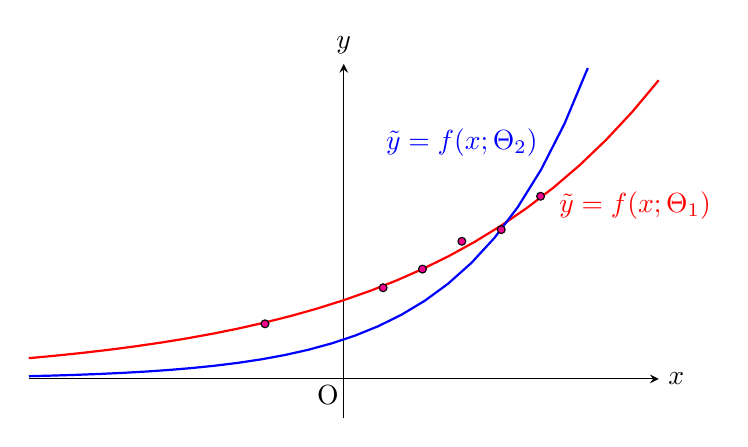
\begin{tikzpicture}[>=stealth]
        \draw[->](-4,0)--(4,0) node[right] {$x$};
        \draw[->](0,-0.5)--(0,4) node[above]{$y$};
        \node at(-0.2,-0.2) {O};
        \draw[draw=red,thick,domain=-4:4] plot(\x,{exp(\x/3)});
        \draw[draw=blue,thick,domain=-4:3.1] plot(\x,{exp(\x/1.5)/2});
        \node at(3.7,2.2) {\textcolor{red}{$\tilde{y}=f(x;\Theta_{1})$}};
        \node at(1.5,3) {\textcolor{blue}{$\tilde{y}=f(x;\Theta_{2})$}};
        \draw[fill=magenta] (1,1.395) circle[radius=0.05];
        \draw[fill=magenta] (1.5,1.748) circle[radius=0.05];
        \draw[fill=magenta] (2,1.896) circle[radius=0.05];
        \draw[fill=magenta] (2.5,2.32) circle[radius=0.05];
        \draw[fill=magenta] (-1,0.7) circle[radius=0.05];
        \draw[fill=magenta] (0.5,1.158) circle[radius=0.05];
    \end{tikzpicture}
\end{center}
これより教師つき学習をすることによって, 今回の例ではモデルは
\begin{eqnarray*}
    \tilde{y} = f(x;\Theta_{1})
\end{eqnarray*}
であることが推定される.
